%% mode: pdflatex

% TEMPLATE for Usenix papers, specifically to meet requirements of
%  USENIX '05
% originally a template for producing IEEE-format articles using LaTeX.
%   written by Matthew Ward, CS Department, Worcester Polytechnic Institute.
% adapted by David Beazley for his excellent SWIG paper in Proceedings,
%   Tcl 96
% turned into a smartass generic template by De Clarke, with thanks to
%   both the above pioneers
% use at your own risk.  Complaints to /dev/null.
% make it two column with no page numbering, default is 10 point

% Munged by Fred Douglis <douglis@research.att.com> 10/97 to separate
% the .sty file from the LaTeX source template, so that people can
% more easily include the .sty file into an existing document.  Also
% changed to more closely follow the style guidelines as represented
% by the Word sample file. 
% This version uses the latex2e styles, not the very ancient 2.09 stuff.


\documentclass[letterpaper,twocolumn,10pt]{article}
\usepackage{usenix}
\usepackage{url}
\usepackage{graphicx}
\usepackage{booktabs}
\usepackage[l2tabu, orthodox]{nag}                % checks the documents of bad habits
\renewcommand{\refname}{REFERENCES} 
\begin{document}

%don't want date printed
\date{}

%make title bold and 14 pt font (Latex default is non-bold, 16 pt)
\title{\Large \textbf Performance gain with variable chunk size in GFS-like file systems}

%for single author (just remove % characters)
\author{
{\rm Zhifeng Yang, Qichen Tu, Kai Fan, Lei Zhu, Rishan Chen, Bo Peng}\\
\{yzf,tqc,fankai,zhulei,crs,pb\}@net.pku.edu.cn\\
Networks lab, Peking University
} % end author

\maketitle

% Use the following at camera-ready time to suppress page numbers.
% Comment it out when you first submit the paper for review.
\thispagestyle{empty}


\subsection*{ABSTRACT}
We have designed and implemented Tianwang File System(TFS), which is a distributed file system much like Google file system(GFS). The system has its origins in our Tianwang search engine and web mining research work. Our system has the same assumptions and the same architectures with GFS. But the key design choice that the chunk size is variable lets our system to adopt simpler system interactions which significantly improves the performance of the record append operation. 

In this paper, we discuss many aspects of our design which are different from GFS, and verify their pros and cons by performance experiments. The experiment results show that the utilization ratio of our record append operation excels GFS by 25\%. And the throughput of record append of TFS is also several times better. 
\section{INTRODUCTION}
\subsection{Background}
With the rapid growth of Web, search engine companies have achieved tremendous successes. We have come into a new era in which who owns the most data and the most powerful data process ability will be the leader of technological innovation. The huge Web is a treasure trove of this new era. As a result, Web information retrieval and Web data mining become more and more popular, and people urgently need a computing environment for Web scale data processing.

TFS(Tianwang file system) is a scalable, distributed file system, which meets the need for data storage and management services in large scale data processing. The system has its origins in our Tianwang search engine~\cite{Tianwang} and web mining research work. There are always lots of difficulties which face researchers who engage in processing large scale data, especially Web scale data. For example, the hardware is unreliable and there are disc and machine failures all the time. Every programmer of distributed applications should consider where to locate data and how to access them. Many of them are just duplicates work already done by someone else. It is worse that the task of implementing an efficient distributed application presents many difficulties even to a senior programmer without much experience in the parallel programming, and their applications are usually inefficient. Moreover, with the growth of the data, we add more and more machines. But these data and resources are not easily shared, and the utilization ratio of these hardware resources is low. All these problems call for a reliable, scalable infrastructure for large scale data computing. And our Tianwang file system is a basic component of such an infrastructure. 
\subsection{Related Works}
The most remarkable and pathbreaking related work is Google file system~\cite{gfs2003}. Google has built a reliable, scalable and high performance distributed file system on inexpensive commodity hardware. Their subsequent publications (\cite{mapreduce}, \cite{bigtable}) make more and more people begin to realize the importance of building such an infrastructure for distributed data-intensive applications. Google's work shows us the rudiments of a super computing platform of the new era.

Another work in progress is a project called Hadoop~\cite{hadoop}. It was a module in Lucene/Nutch java project to provide the similar function of Google file system and mapreduce. As a active open source project, it helps us to think more deeply of the work from the technical view. Hadoop does not support concurrent atomic record append, which is a very important operation. Files are created and written by one writer and can not be modified any more. KFS~\cite{kfs} is another recent project implemented in C++ programming language. It has more features than Hadoop supports. An interesting feature is that it can be integrated with Hadoop using Hadoop's file system interfaces. Microsoft's Dryad system~\cite{Dryad2007} is indicative of their effort towards the same direction, though public paper is not yet available.

Our long-term goal is to build an infrastructure for processing large scale data, TFS is our first step to the goal.
\section{SYSTEM OVERVIEW}
\subsection{Architecture}
We have followed the same architecture with Google file system. A TFS cluster consists of a single \emph{master} and multiple \emph{chunkservers} and is accessed by multiple \emph{clients}. 

Files are divided into variable-size chunks. Each chunk is identified by an immutable and globally unique 64 bit chunk handle assigned by the master at the time of chunk creation. Chunkservers store chunks on local disks as Linux files and read or write chunk data specified by a chunk handle and byte range. For reliability, each chunk is replicated on multiple chunkservers. By default, we store three replicas, though users can designate different replication levels for different files.

The master maintains all file system metadata. This includes the namespace, access control information, the mapping from files to chunks, and the current locations of chunks. It also controls system-wide activities such as garbage collection of orphaned chunks, and chunk migration between chunkservers. Each chunkserver periodically communicates with the master in \emph{HeartBeat} messages to report its state and get back instructions. 

TFS client code linked into each application implements the file system API and communicates with the master and chunkservers to read or write data on behalf of the application. Clients interact with the master for metadata operations, but all data-bearing communication goes directly to the chunkservers. 

The system is designed to minimize the master's involvement in file accessing operations. We do not provide the POSIX API. Besides providing the ordinary read and write operations, like GFS, we have also provided an atomic record append operation so that multiple clients can append concurrently to a file without extra synchronization between them. And we realize that the record append operation is the key operation we should optimize so our system interactions is different from GFS and we expect better performance of record append than GFS. 
\subsection{Chunk Size}
In Google file system, a file is divided into fixed-size chunks(64 MB). In GFS' design, when a client use record append operation to append data, the system checks to see if appending the record to the current last chunk would cause the chunk to exceed the maximum size. If so, it pads all the replica of the chunk to the maximum size, and replies to the client indicating that the operation should be retried on the next chunk. (Record append is restricted to be at most one-fourth of the maximum chunk size to keep worstcase fragmentation at an acceptable level.) On the occurrence of write failure, this at-least-once semantic can lead to duplicated records and incomplete records.

In TFS, the chunks of a file have variable sizes. With our different system interactions which will be addressed in details in the following subsections, this design choice makes our record append operation nobler and more efficient. Padding data, record fragments, record duplications do not exist in our system. Of course, this improvement brings some problems and concerns. For instance, every data structure of chunk need a chunk size attribute, which increases the memory overhead. Despite this drawback, we expect that read and record append operations that are key operations in our system can benefit from this design choice. 
\subsection{Read Operation}
During a read operation, the client exchanges messages with the master and gets the current locations of chunks it wants to read from. Then it communicates with the chunkservers and gets the data. This process is different due to the different chunk size strategy. 

In Google file system, using the fixed chunks size, the client translates the file name and byte offset specified by the application into a chunk index within the file. Then, it sends the master a request containing the file name and chunk index. The master replies with the corresponding chunk handle and locations of the replicas. The client caches this information using the file name and chunk index as the key.

The client then sends a request to one of the replicas, most likely the closest one. The request specifies the chunk handle and a byte range within that chunk. Further reads of the same chunk require no more client-master interaction until the cached information expires or the file is reopened.

In our system, because the chunk size is variable, the client can not translate the byte offset into a chunk index directly. It has to know all the chunks' sizes of the file before deciding which chunk should be read. Our strategy is simple, when a client opens a file using read mode, it also gets all the chunks' information, including chunk handle, chunk size and locations, from the master. When the client needs to read some data, it can use these informations to get the proper chunk. Although this strategy is determined by the fact of variable chunk size, its advantage is that the client need only to communicate with the master once for reading the whole file, which is much efficient than GFS' original design.

The disadvantage, though, is that when a client has opened a file for reading, later appended data by the other clients is invisible to this client. But we think this is acceptable, considering the most files in our applications are created and appended once, and read by data processing applications many times without modifications. If in any situation this problem becomes critical, it can be easily overcome by set a expired time for the chunks' information and refresh it when invalid. So the novelty of file's metadata is under control. 
\subsection{Record Append Operation}
High performance of the record append operation is the most important factor that affects our design decisions. Because a write or an append operation is performed at all the chunk's replicas, the system must maintain the consistency among replicas. 


In Google file system, they use leases to maintain a consistent mutation order across replicas. The master grants a chunk lease to one of the replicas, which we call the \emph{primary}. The primary picks a serial order for all mutations to the chunk. All replicas follow this order when applying mutations. Thus, the global mutation order is defined first by the lease grant order chosen by the master, and within a lease by the serial numbers assigned by the primary.

When a client use record append operation to append data, the system checks to see if appending the record to the current last chunk would cause the chunk to exceed the maximum size. If so, it pads all the replica of the chunk to the maximum size, and replies to the client indicating that the operation should be retried on the next chunk. If a record append fails at any replica, the client retries the operation. As a result, replicas of the same chunk may contain different data possibly including duplicates of the same record in whole or in part. GFS does not guarantee that all replicas are bytewise identical. It only guarantees that the data is written at least once as an atomic unit. 

In our system, we do not use the complex lease mechanism. Append operation is based on chunk level. In Figure~\ref{fig:tfswrite}, we illustrate this process by following the control flow of an append through these numbered steps.
\begin{figure}[t]
\begin{center}
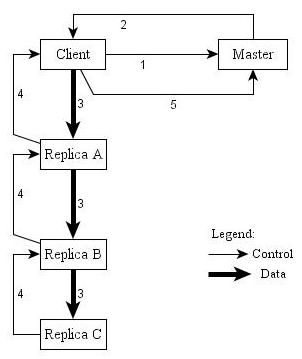
\includegraphics[width=0.38\textwidth]{tfs_write}
\end{center}
\caption{Append Control and Data Flow}
\label{fig:tfswrite}
\end{figure}
\begin{enumerate}
\item The client asks the master to allocate a new chunk to append data to.
\item The master allocates a new chunk handle and choose several chunkserver as chunk replicas according to the workloads of all the chunkservers at that moment. It records this new chunk in its data structures and returns the chunk handle and locations to the client.
\item The client sends the append command and the appended data to the nearest chunkserver, then the first chunkserver send the data and command to the next chunkserver\ldots The data is sent by pipeline. 
\item The message about whether a chunkserver's replica is successfully written is sent back to the client by pipeline. 
\item If at least one of the chunkservers is successfully written, the client send message of success and the successfully written replicas to the master, then the master modifies its metadata. If none of the replicas is written successfully, the client can retry the operation for several times before eventually it tells the master to abandon the allocated chunk and throws the exception to the application. The orphan chunks will be deleted by the system's garbage collection mechanism. 
\end{enumerate}

In our system, every appending chunk has only one writing client, but we allow multiple chunks of a file to be appended simultaneously. The client itself in fact plays the role of the \emph{primary}. This is our different mechanism to support concurrent record appends. But it is false that every record append operation of applications will generate a new chunk. In fact the client library bundles up multiple appended data and generate a chunk in batch. Because there is cached appending data, the client's exception will lead to lost of some data. We supply a flush API to allow the applications who can not tolerate such situation to make sure the critical data has been written to the chunkservers.

In GFS, the aggregate record append performance is limited by the network bandwidth of the chunkserver that store the last chunk of the file, independent of the number of clients. But in our system, the more chunkservers and concurrent clients, the higher the aggregate performance, the only limit is aggregate bandwidth between clients and chunkservers. 
\subsection{Write Operation}
In Google file system, write operation use the same lease mechanism as record append operation. So concurrent write to the same region is allowed, but the result is undefined. The region is most likely made up of fragments from different write operation. However, as long as the write operation is successful, the lease mechanism can guarantee the replicas of the same chunk are consistent. 

We consider that it is not necessary to adopt the complex mechanism in order to allow concurrent write operation. First, although the results of the concurrent writes operations are consistent, it is useless. Secondly, for the existence of record append operation, write operation is mainly used to overwrite the existing chunks. In practice, overwrite operation is rare, and concurrent overwrite operation is even more rare. For the sake of the rarely used write operation, they lose the opportunity to improve the performance of record append operation because both of these operations use the same lease mechanism. The loss outweighs the gain. 

In our system, we treat write and record append distinctly. They are implemented using different system interactions so we can adopt more efficient way to implement the record append operation. We simply do not allow concurrent write operations. When a client opens a file as write mode, the whole file is locked exclusively. 
\subsection{Implications for Applications}
The GFS record append operation can generate paddings, duplicated records, incomplete records and inconsistent replicas. So the GFS applications have to accommodate these with a few other techniques: relying on appends rather than overwrites, checkpointing, and writing self-validating, self-identifying records.

Our append operation with append-exactly-once semantics is noble, and we only require the applications to rely on appends rather than overwrites. Practically all our applications mutate files by appending rather than overwriting. In one typical use, many writers concurrently append to a file for merged results or as a producer-consumer queue. Then many other readers concurrently read the different region of the file, process the data and concurrently append the result to another file. 

Like GFS, TFS' record append cannot guarantee the sequence of the operations. That means, if an application sequentially append two record into a file, it should not expect they are stored in the file beside each other. However, it is true the first appended record will have smaller offset than the second one. 
\section{EXPERIMENTS}
We measured performance on a TFS cluster consisting of one master, nine chunkservers, and ten clients. Note that this configuration was set up for ease of testing. Typical clusters may have hundreds of chunkservers and hundreds of clients.

The master and chunkserver machines are Dell 2850 configured with two 2.80GHz Intel Xeon processors, 2GB of memory, six 7200 rpm Ultra SCSI drives configured as one software RAID-0 volume. All the client machines are the same as above except the memory is 4GB. And all these machines have a 1 Gbps full-duplex Ethernet connection to a Dell 2748 1 Gbps switch. 

\subsection{Master Operation}
This experiment is set up to test the performance of the master operations, and whether the single master architecture will be the bottleneck of the whole system. 

Ten clients simultaneously send RPC request to the master. Each operation is repeated for 10000 times. The evaluation measure we use is operations per second(Ops/s). For each operation we calculate its Ops/s. 

Table~\ref{tab:chunkop} shows the master's Ops/s of chunk operations. The \emph{getChunksInfo} is the key operation that affects the whole system performance. We set up different numbers of chunks to represent different typical file size in real system to test it. The results show the master can easily handle thousands of \emph{getChunksInfo} requests every second. And the Ops/s of some of the simple operations is extremely high, e.g. \emph{abandonAddChunk}. 
\begin{table}
  \centering
  \begin{tabular}{l|r}\toprule[1.5pt]
    Chunk Operation&Ops/s\\ \midrule
    addChunk&2933\\ \midrule
    completeWrittenChunk&7663\\ \midrule
    abandonAddChunk&11403\\ \midrule
    getChunksInfo(0 chunk)&8782\\ \midrule
    getChunksInfo(20 chunks)&2578\\ \midrule
    getChunksInfo(50 chunks)&1225\\ \midrule
    getChunksInfo(100 chunks)&683\\ \midrule
    getChunksInfo(150 chunks)&453\\ \midrule
    getChunksInfo(200 chunks)&350\\ \midrule
  \end{tabular}
  \caption{Master Chunk Operations}
  \label{tab:chunkop}
\end{table}
%\begin{table}
%  \centering
%  \begin{tabular}{l|r}\toprule[1.5pt]
%    File Operation&Ops/s\\ \midrule
%    createFile&620\\ \midrule
%    renameFile&311\\ \midrule
%    removeFile&2252\\ \midrule
%    getFileInfo&609\\ \midrule 
%    open&3246\\ \midrule
%    close&2881\\ \bottomrule
%  \end{tabular}
%  \caption{File Operations}
%  \label{tab:fileop}
%\end{table}
%\begin{table}
%  \centering
%  \begin{tabular}{l|r}\toprule[1.5pt]
%    Directory Operation&Ops/s\\ \midrule
%    createDirectory&230\\ \midrule
%    renameDirectory&121\\ \midrule
%    removeDirectory&5942\\ \bottomrule
%  \end{tabular}
%  \caption{Directory Operations}
%  \label{tab:dirop}
%\end{table}

In the real running system, these operations are interleaving. We designed a simulation workload of a real system, following the ratio of different type of operations indicated in Google's experiments(in \cite{gfs2003} section 6.3.4). Ten clients concurrently execute the sequence with 42000 operations. The test shows that on average every client consumed about 122 seconds to finish the operations. That is, the workload of the master is 3443 operations per second. In Google's paper, they mention that the rate of operations send to their master is around 200 to 500 operations per second. Our master can easily keep up with this rate. And there is no bottleneck even for the workload of 3000 Ops/s. 
\subsection{Read Buffer Size}
In our read operation, the client uses a buffer to receive the data from chunkservers. The buffer size determines the size of data transferred to the client in each communication. In this experiment, we test how different buffer size will affect the performance of read. 

Using different read buffer size, one client reads a 1GB region from a file. Figure~\ref{fig:buffersize} shows different buffer size and its read rate. The read rate reaches its maximum when the size is around 1024KB, and becomes flat. So we choose 1024KB as the default value of the read buffer size. 
\begin{figure}
\centering
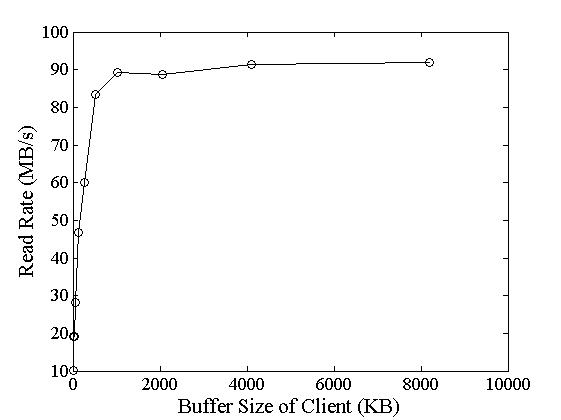
\includegraphics[width=0.5\textwidth]{buffersize}
\caption{Read Buffer Size}
\label{fig:buffersize}
\end{figure}

\subsection{Reads and Record Appends}
Because all our clients and servers machines are connected to one switch, to get the theoretical network limits, we run all the clients as different threads on one client machine. So the limit of network throughput of all these clients is bound to 125MBps. 

N clients read simultaneously from the file system. Each client reads a randomly selected 4 MB region from an 18 GB file. This is repeated 256 times so that each client ends up reading 1 GB of data. Figure~\ref{fig:readtest} shows the aggregate read rate for N clients. Note that the limit peaks at an aggregate of 125 MB/s when the client's 1 Gbps network interface gets saturated. The aggregate read rate reaches 90 MB/s, about 72\% of the 125 MB/s network limit. The efficiency of single client drops sometimes most likely because as the number of readers increases, so does the probability that multiple readers simultaneously read from the same chunkserver.
\begin{figure}
\centering
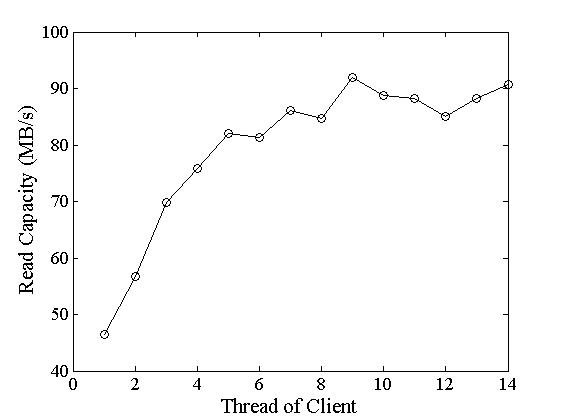
\includegraphics[width=0.5\textwidth]{readtest}
\caption{Aggregate Read Rate}
\label{fig:readtest}
\end{figure}
Figure~\ref{fig:appendtest} shows the record append performance. N clients append simultaneously to a single file. Performance is limited by the aggregate bandwidth of links between the chunkservers and clients. That is 125 MBps in our network topology. The aggregate append rate reaches 95 MB/s, about 75\% of the 125 MB/s network limit. In another experiment , we run multiple clients on different machines. The result shows that aggregate append rate can easily exceed 380MB/s, which is a demonstration of our expectation that out record append performance will not drop due to the network limit of one chunkserver like in GFS. 
\begin{figure}
\centering
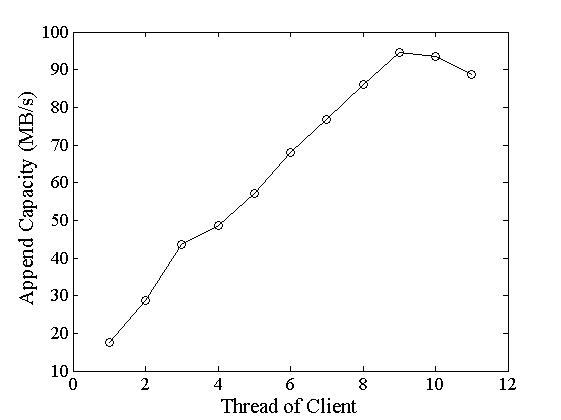
\includegraphics[width=0.5\textwidth]{appendtest}
\caption{Aggregate Record Append Rate}
\label{fig:appendtest}
\end{figure}

In contrast to our performance, the read and record append operations in Google file system can reach 75\% and 50\% of the theoretical limit, separately. So our record append performs much better. During the entire test, the rate of CPU of that client machine maintained less than 5\%, so there is no contest of CPU which may lead to the deviation of the results.
\section{CONCLUSION}
The Tianwang file system demonstrates our effort to build an infrastructure to support large scale data processing. Although our system has the same assumptions and the same architectures with Google file system, the key design choice that the chunk size is variable, which is different from GFS, lets our system to adopt different system interactions for record append operation. And the experiment results show that our design significantly improves the record append performance by 25\%. We believe the design may apply to other similar data processing infrastructure.

We observed that using the same system interaction for both write and record append is a shortcoming in GFS and restricts the possibility of digging for more better append performance, which led to our different points in the design space. Our chunk size of file is variable and record append operation is based on chunk level. Because of this, the aggregate record append performance is no longer limited by the network bandwidth of the chunkservers that store the last chunk of the file. 

%During the What i have learned from the system design: distributed system debug, log, 
Our system is going to be used by our research group to manage the largest Chinese Web archive system~\cite{infomall}. And we are working on a distributed computing environment to support data processing files upon our file system.
\section{ACKNOWLEDGMENTS}
This work is supported by National Grand Fundamental Research 863 program of China under Grant No. 2006AA01Z196, National Natural Science Foundation of China under Grant No. 60672171. And we wish to thank Conglei Yao for his valuable comments and suggestions to the paper. 

{\footnotesize \bibliographystyle{acm}
\bibliography{myBib}}

\end{document}







